\section{Listening Data Construction}
\label{sec:data}
% Section role: explain how paired media, descriptions, and labels are constructed.

\begin{figure*}[t]
\centering
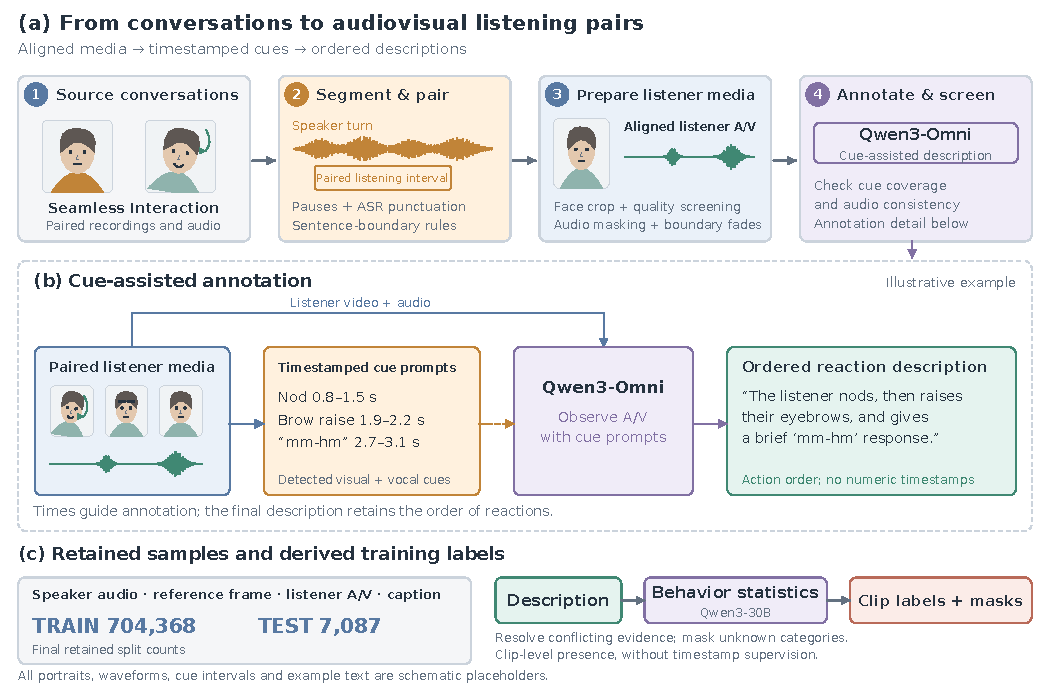
\includegraphics[width=\textwidth]{F2_data.pdf}
\caption{\figdraft{F2: Data construction and cue-assisted annotation} Seamless conversations are segmented and paired before listener media processing. Listener audiovisual media and timestamped reaction cues guide Qwen3-Omni to produce an ordered description without numerical timestamps. Each sample links the input conditions, listener targets, and description. Text-based behavior extraction and conflict masking produce clip-level training labels. Example media, cue intervals, and descriptions are schematic; the reported resource counts differ from the AV training selection.}
\label{fig:data}
\end{figure*}
\subsection{Role-Aware Pair Construction}
\label{sec:pairing}

We construct 2--12-second listening clips from Seamless
conversations~\cite{seamless}, pairing the current speaker's
audio with a listener reference frame and synchronized
listener audio and video. Transcripts, word timings,
speech activity, and pauses guide segmentation toward
complete sentences. Roles switch when the listener takes
the conversational floor, while brief vocal backchannels,
including overlapping feedback, remain part of listening.
\Cref{fig:data} summarizes the pipeline.

Listener videos are screened, corrected for orientation
where needed, and cropped consistently for reaction
detection and annotation. Listener audio is extracted
from the participant's separate track over the same
interval. Officially annotated vocal regions are retained
with short margins and boundary fades; the remaining
audio is set to zero, preserving duration and audiovisual
alignment.

\subsection{Cue-Assisted Reaction Annotation}
\label{sec:annotation}

To reduce omissions of brief reactions, we extract visual
and vocal cues and provide their categories and temporal
intervals to Qwen3-Omni~\cite{qwen3omni}, together with the
listener audio and video. The model is prompted to describe
the reactions in their observed order without numerical
timestamps.

We then use Qwen3-30B-A3B-Instruct-2507~\cite{qwen3} to
extract clip-level behavior labels from these descriptions.
Supported categories provide positive labels, while
unmentioned categories receive weak-negative labels only
after completeness checks. Uncertain or conflicting labels
are masked, as detailed in \cref{sec:event}.

\subsection{Dataset Statistics}
\label{sec:data-statistics}
% Paragraph role P07: 样本与规模
Each sample links the current speaker audio, the listener's first frame, aligned listener video and audio, and a reaction description, together with source and temporal metadata. The retained resource contains 704,368 training samples and 7,087 test samples. The AV generation model uses a separately selected training set, specified in \cref{sec:setup}; these counts do not denote the same training manifest. Data and annotation quality checks are organized in \cref{sec:validation}.
% Candidate 1: dataset comparison. Caption is below the table as requested.
% TBD means unverified in this writing pass, not unavailable or unreported.
\begin{table*}[t]
    \centering\small
    \begin{tabularx}{\textwidth}{@{}Yccc@{}}
    \toprule
    Dataset & \makecell{Listening\\organization} &
    \makecell{Separate speaker/\\listener audio} & Paired samples \\
    \midrule
    ViCo~\cite{vico} & Dedicated & \pending & 483 clips \\
    RealTalk~\cite{realtalk} & General dialogue & \pending & \pending \\
    Seamless~\cite{seamless} & General dialogue & \on & \pending \\
    SpeakerVid-5M (listening)~\cite{speakervid} & Dedicated branch & \off & \pending \\
    ResponseNet~\cite{omniresponse} & General dialogue & \on & 696 conversations \\
    GLARE~\cite{glare} & Dedicated & \pending & 107,149 clips \\
    \midrule
    Ours & Dedicated & \on & 711,455 clips \\
    \bottomrule
    \end{tabularx}
    \caption{【Candidate 1】Comparison of data resources. Separate audio denotes participant-specific tracks for both speakers and listeners; the SpeakerVid-5M listening branch pairs speaker audio with silent listener video. Conversation counts and segmented-clip counts use different units. Ours counts the retained training and test pairs.}
    \label{tab:dataset-comparison}
    \end{table*}
    

% Candidate 2: method scope and generated modalities, not a performance ranking.
\begin{table*}[t]
    \centering\small
    \begin{tabularx}{\textwidth}{@{}Yccc@{}}
    \toprule
    Method & \makecell{Listening\\modeling} & Joint A/V & Generated output \\
    \midrule
    CustomListener~\cite{customlistener} & Dedicated & \NA & Visual \\
    DiffListener~\cite{difflistener} & Dedicated & \NA & Visual \\
    GLARE~\cite{glare} & Dedicated & \NA & Visual \\
    INFP~\cite{infp} & Included & \NA & Visual \\
    OmniResponse~\cite{omniresponse} & Included & \off & Audio + visual \\
    OmniPersona~\cite{omnipersona} & Included & \on & Audio + visual \\
    \midrule
    Ours & Dedicated & \on & Audio + visual \\
    \bottomrule
    \end{tabularx}
    \caption{【Candidate 2】Comparison of generation settings. Dedicated methods focus on listening; Included methods also model listening within broader interaction tasks. Joint A/V denotes joint audio--video synthesis; OmniResponse synthesizes audio through TempoVoice. Outputs list generated modalities, excluding supplied audio.}
    \label{tab:method-comparison}
    \end{table*}
    

% Candidate 3: our retained train/test resource; not the 284,218-clip AV selection.
% Example category rows must be replaced/expanded after the vocabulary is frozen.
% Neither the training Event vocabulary nor the seven evaluation classes defines
% the full dataset taxonomy automatically. Counts below are intentionally TBD.
\begin{table*}[t]
    \centering\small
    \begin{tabularx}{\textwidth}{@{}lYrrr@{}}
    \toprule
    Modality & Behavior category & Train pairs & Test pairs & Total pairs \\
    \midrule
    Visual & Head nodding & \pending & \pending & \pending \\
           & Smiling & \pending & \pending & \pending \\
           & $\ldots$ & $\ldots$ & $\ldots$ & $\ldots$ \\
    Vocal & Audible laughter & \pending & \pending & \pending \\
          & $\ldots$ & $\ldots$ & $\ldots$ & $\ldots$ \\
    \midrule
    \multicolumn{2}{@{}l}{Number of visual categories} & \multicolumn{3}{r@{}}{\pending} \\
    \multicolumn{2}{@{}l}{Number of vocal categories} & \multicolumn{3}{r@{}}{\pending} \\
    \multicolumn{2}{@{}l}{Total number of categories} & \multicolumn{3}{r@{}}{\pending} \\
    \midrule
    \multicolumn{2}{@{}l}{All pairs (unique within each split)} & 704,368 & 7,087 & 711,455 \\
    \bottomrule
    \end{tabularx}
    \caption{【Candidate 3】Category distribution and split sizes of our retained data. Category rows illustrate the layout pending the final vocabulary and counts. Each pair is counted once per category and may contain multiple categories, so category counts need not sum to the dataset total.}
    \label{tab:data-statistics-candidate}
    \end{table*}
    
\cnnote{感觉可以去掉。如果保留的话要补充：数据总量xx条xxh、标柱类别数xx种}{}
